%% This is an example first chapter.  You should put chapter/appendix that you
%% write into a separate file, and add a line \include{yourfilename} to
%% main.tex, where `yourfilename.tex' is the name of the chapter/appendix file.
%% You can process specific files by typing their names in at the 
%% \files=
%% prompt when you run the file main.tex through LaTeX.
\chapter{DressCode}\label{sec:DressCode}

\begin{center}
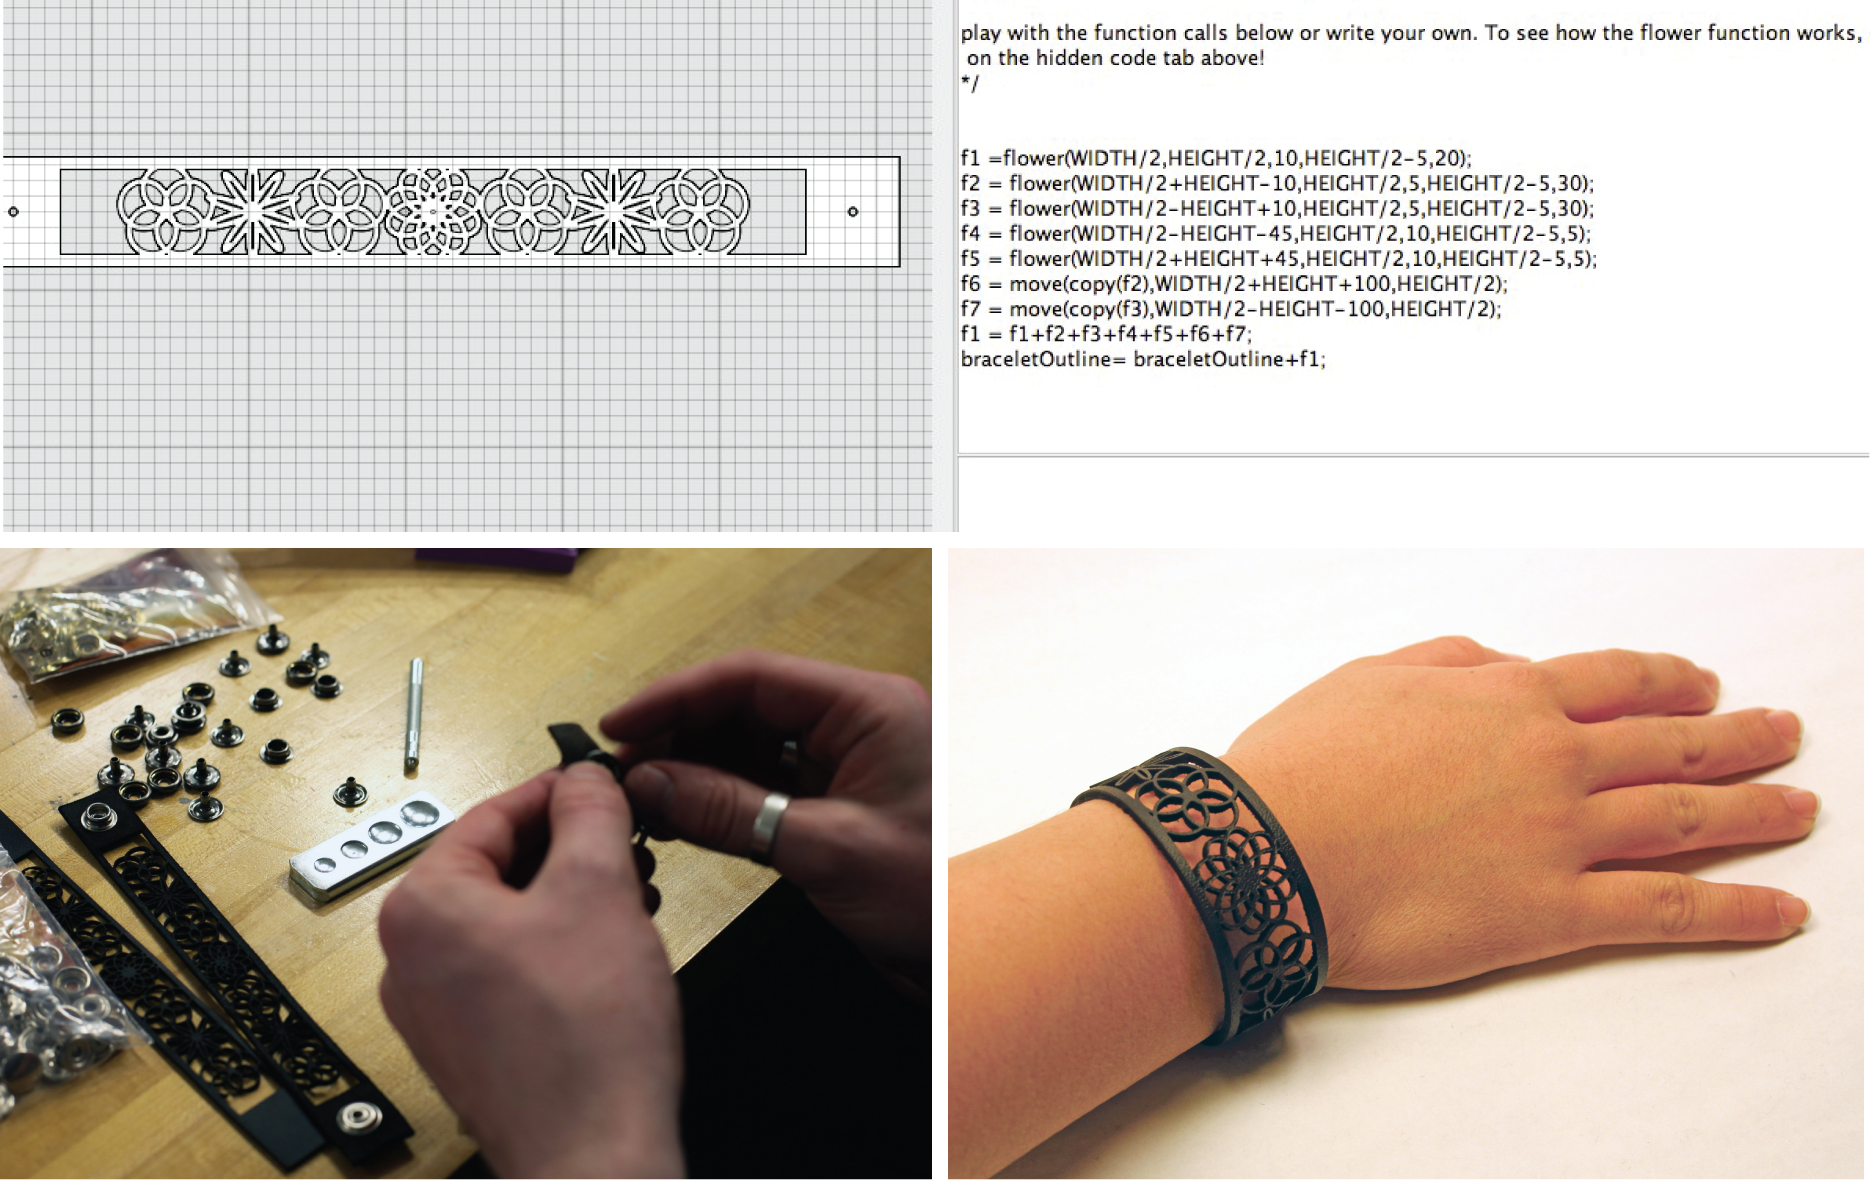
\includegraphics[width=6.5in]{images/dressCode_main.png}
\end{center}


The preliminary work of Codeable Objects and Soft Objects clearly demonstrated that algorithmic craft offers a compelling opportunity for personal, creative expression through programming. My goal following these projects was to address some the limitations present in these preliminarily projects by developing a stand-alone programing environment and design tool. The resulting software, DressCode is a tool developed expressly to support new programmers in open-ended casual computational design for digital fabrication. To evaluate Dress Code, I conducted two separate day long workshops, one with experienced programmers and designers, and one for young people who were new to programming. I also worked with FUSE, an out of school STEAM exploration program to develop a set of online activities using DressCode, which is currently in the preliminary stages of evaluation.	 

\section{Design principles}
Based on the success of the prior fashion workshop, and my continued interest in exploring applications that appeal to women and girls, I decided to focus on computational fashion design and the fabrication of wearable artifacts in the development of DressCode. After reflecting on the potential limitations of this focus however, I decided to develop DressCode as a more open-ended computational design tool that could support the creation of a variety of artifacts, rather than just fashion. To preserve the emphasis on fashion, the majority of the example projects and artifacts I created with DressCode for this thesis were fashion-oriented. The workshops I conducted, as well as the curriculum I helped develop also had an emphasis on fashion or wearable artifacts.

By building my own software, I sought to improve on the preliminary programming libraries in three key areas. First, DressCode contains its own programing language. The DressCode language has a simplified syntax and contains a limited set of textual programming methods, allowing people with little-to-no prior programming experience to working with the language quickly and effectively. Second, the DressCode environment is designed to equally prioritize textual programing and visual design and manipulation. To that end, the software has a two-panel development environment that displays a graphic two-dimensional (2-D) rendering of the user�s current design in the first panel, and their code in the second. As a user makes changes to their code, the effects on the design are rendered in the graphic panel. Finally, DressCode contains functionality that is specific to digital fabrication and algorithmic craft. The tool allows for a variety of methods to translate one's design to a tool-paths for fabrication machines. In addition, the API contains programing methods that support the creation of forms and patterns that are suitable for fabrication, with minimal effort on the part of the user.  The goal of designing a software 2-panel programing and design environment, with a specialized programing language and immediate support for digital fabrication was to assist non-programmers in independently making design decisions with programing. In short, I wanted to make it as easy as possible for people to decide on their own desired style or aesthetic, and then realize it by writing their own code. The following section describes the features of the DressCode software in greater detail.

\section{Tool description}
I've divided the description of DressCode into three sections: the programing syntax and drawing API, the interface design, and the process of going from DressCode to a fabrication machine.
\subsection{Programing Language}
The DressCode programing language is interpreted with semantic functionality that is simulated through a Java-based library.  We relied on the ANTLR framework to generate the necessary lexing and parsing methods for the language, and developed the semantic functionality using java and the java openGL (JOGL). When a program is run in DressCode, the raw script is first tokenized and then parsed to generate an abstract syntax tree (AST). During this phase, all user-generated function definitions are stored in memory. If any parsing errors are encountered, they are output to the console as "compiler errors". Assuming the parse is successful, DressCode then walks the resultant AST and attempts to execute the semantic functionality of the program (figure:\ref{fig:interpreter_structure}.) After being excecuted, the resultant design is rendered on the display panel. Any runtime errors are displayed in the output console. For most programs, this process is instantaneous, however some programs with complex operations require several seconds to be excecuted. 
  \begin{center}
\begin{figure}[h!]
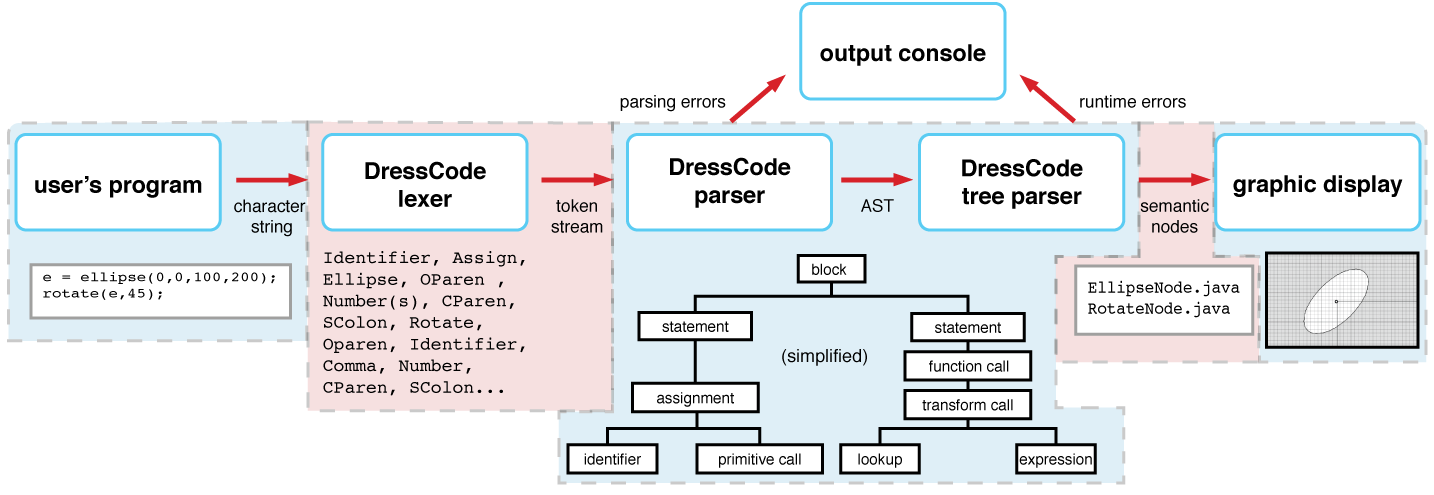
\includegraphics[width=6.5in]{images/interpreter_structure_horz.png}
\caption{Interpreter structure}
\label{fig:interpreter_structure}
\end{figure}
\end{center}
The language is imperative in nature, with statements being executed in the order in which they are read. The exception to this is user defined functions, which may be defined at any point in the program, and called before they are defined. Each statement in DressCode must be terminated by a semicolon. I spent some time experimenting with terminating statements with newlines, similar to whitespace sensitive languages like Python, as I thought this might be more conducive to novice use. Unfortunately, the implementation of selective whitespace recognition is a challenging task to define in a grammar, so while we were able to develop a version of DressCode that recognized statements terminated by a line break, it would have taken significant time to develop this functionality to a level of robustness appropriate for user testing. For the short term, we have opted for a syntax requiring semicolons, however we plan to continue to explore newline statement termination in the future. 

\subsubsection{Language Structure}
DressCode supports number, string, boolean, and drawable datatypes (figure \ref{fig:basic_datatypes}.) The first four of these types are relatively standard in comparison to conventional programing languages. Numbers include integers and floating point values. Strings include any sequence of characters enclosed in double quotations. Booleans have two possible values: true, and false. Drawables are a special type, discussed in detail in the API description below. DressCode also contains a list data structure, which can store multiple kinds of datatypes.
\begin{center}
%\begin{figure}
\begin{lstlisting}
myString = "hello";  //string
myNum = 10.4;  //number
numbermyBool = true;  //boolean
myList = [10,11,false,"world"];  //list with multiple data types
println(myList[3]); //prints world
\end{lstlisting}
%\caption{basic datatypes}
%\label{fig:basic_datatypes}
%\end{figure}
\end{center}

Variable identifiers in DressCode must begin with a letter which followed by 0 or more letters or digits. Variables can be initialized through assignment, or declared and assigned later in the program. All assignment in DressCode is dynamically typed, and variables can be assigned to datatypes that differ from their original assignment at any point. %(figure \ref{fig:variable_assignment}.)

\begin{center}
%\begin{figure}
\begin{lstlisting}
s1 = "hello";
s2 = "world";
s3; //variable without initial assignment

s3 = s1+" "+s2; 
println(s3); //prints hello world

n1 = 2;
n2 = 2.5;
println(n1+n2*10); // returns 27.0
\end{lstlisting}
%\caption{variable assignment.}
%\label{fig:variable_assignment}
%\end{figure}
\end{center}

The  language also contains support for basic expressions, as well as block statements, including conditionals, loops and user-defined functions. For mathematical expressions, standard order of operations is maintained, unless parentheses are introduced. All block statements are signified by a keyword followed by a colon, and terminated with the end keyword which is not followed by a semicolon.Conditionals are defined with the if keyword, and may an optional else clause and  zero or more else if clauses. %(figure: \ref{fig:conditionals}.)

\begin{center}
%\begin{figure}
\begin{lstlisting}
//if statement 
if 5<10:
println("true"); //prints true
end

//if statement with else if and else clause
i=10;
if i<10:
println("less than 10");
else if i==10:
println("equals 10"); //prints equals 10
else:
println("greater than 10");
end
\end{lstlisting}
%\caption{conditional definitions}
%\label{fig:conditionals}
%\end{figure}
\end{center}

There are two possible loop statements: repeat statements and while statements. Repeat statements begin with the repeat keyword and are followed by a the initialization: a variable identifier with a numerical assignment, followed by a colon and the test, a number that determines the point at which the repeat statement will terminate. By default, all repeat statements have an update value of 1, however this can be modified by following the test value with "add" and a 3rd value specifying the update condition. While loops are initialized with the while keyword and followed by a test condition.%(figure: \ref{fig:loops}.) 

\begin{center}
%\begin{figure}
\begin{lstlisting}
//repeat statement
repeat i=0:10:
ellipse(0,i*10,10,10); //draws a vertical row of 10 ellipses
end

//repeat with modified update condition
repeat i=0:10 add 2:
println(i); //will print 0,2,4,6,8
end

//while statement
c=0;
while c < WIDTH:
ellipse(c,10,20);
c = c+20;
end
//draws a row of ellipses that span the width of the canvas
\end{lstlisting}
%\caption{loop definitions}
%\label{fig:loops}
%\end{figure}
\end{center}

Finally, custom functions are defined with the def keyword, followed by an identifier and a set of parentheses containing 0 or more arguments separated by commas. The function block is terminated with the end keyword like all other block statements. Just like general assignments, functions arguments are dynamically typed. Functions, loops and conditionals all have their own scope and will prioritize identifiers based on that, however if they cannot locate an identifier within their own scope, they will look for it in the level above.
\begin{center}
%\begin{figure}
\begin{lstlisting}
//basic function defintion
def foo(a,b,c):
println(a+b+c);
end

//function call
foo(1,2,3);  //prints 6

//function with return statement
def bar(a,b,c):
return(a*b*c);
end

result = bar(4,5,6)); 
println(result);//prints 120
\end{lstlisting}
%\caption{loop definitions}
%\label{fig:loops}
%\end{figure}
\end{center}

\subsubsection{Drawing API}
 The API is organized around the creation and transformation of 2D shape primitives. By duplicating and manipulating these primitives in a structured manner, it is possible to generate complex and interesting designs from simple forms. The API is composed of three primary main categories, divided by functionality: shape primitives, shape transforms, shape booleans, math operations and property access. A selection of the primary methods from each of these categories is detailed in figure \ref{fig:api_table}. 

  \begin{center}
\begin{figure}[h!]
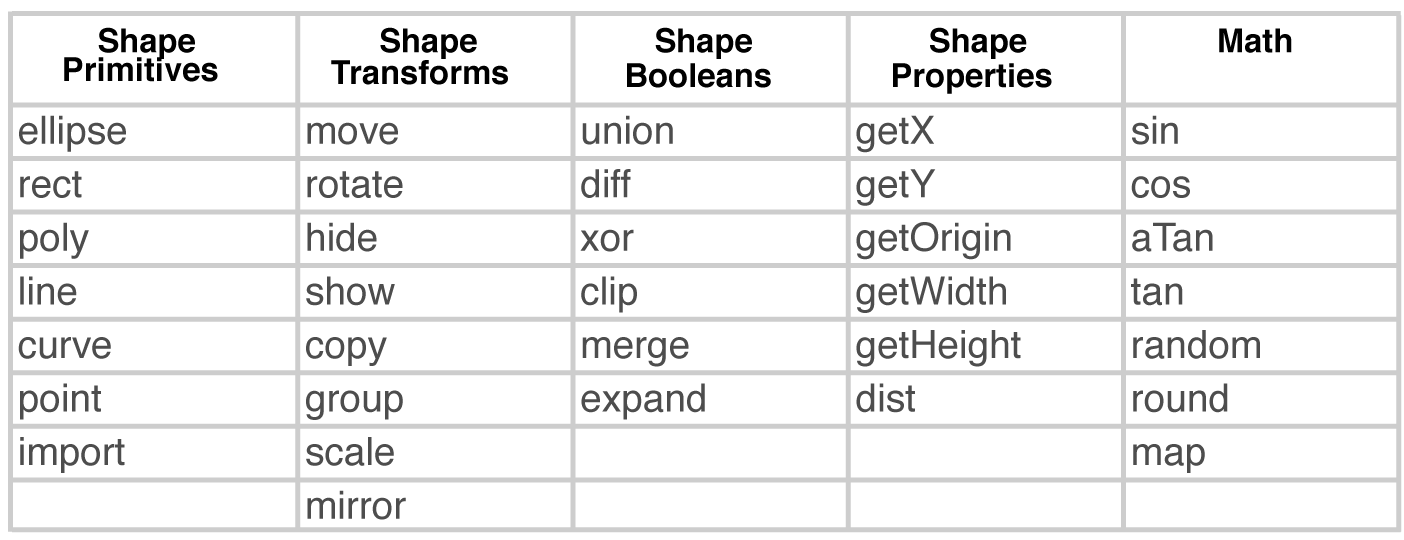
\includegraphics[width=6.5in]{images/api_table.png}
\caption{A selection of methods from the DressCode API}
\label{fig:api_table}
\end{figure}
\end{center}

DressCode shape primitives currently serve as the primary means of drawing (figure: \ref{fig:shape_primitives}.) The simplest primitive is a point, initialized two numerical parameters that denote the x and y coordinates. All closed-shape primitive methods (ellipses, rectangles and polygons) require an argument of either two x,y coordinates, or a point. This coordinate defines the origin of the shape and determines where  the shape will be drawn on the canvas. Ellipses and rectangles have an additional two optional parameters which specify width and height. If only two arguments are provided, the ellipse or rectangle will be drawn with a default width and height; if three arguments are given, the width and height will be the same. Polygons also have two optional parameters following the x and y origin coordinates, however they specify number of sides and length of each side, rather than width and height. Lines can be initialized either as four numerical values, specifying start and end x and y coordinates, two points, or as a vector, with a origin point,  a magnitude, and a heading in degrees. Curves are defined by a set of four points or eight coordinates, which determine the start, first control point, second control point and end point of a 4-point bezier curve. One other method of primitive generation was added in at the request of some of our early users: vector paths stored in Scalable Vector Graphics (SVG) format can be imported and drawn in the DressCode environment, and used in conjunction with primitive transformation and boolean methods.  

 \begin{center}
\begin{figure}[h!]
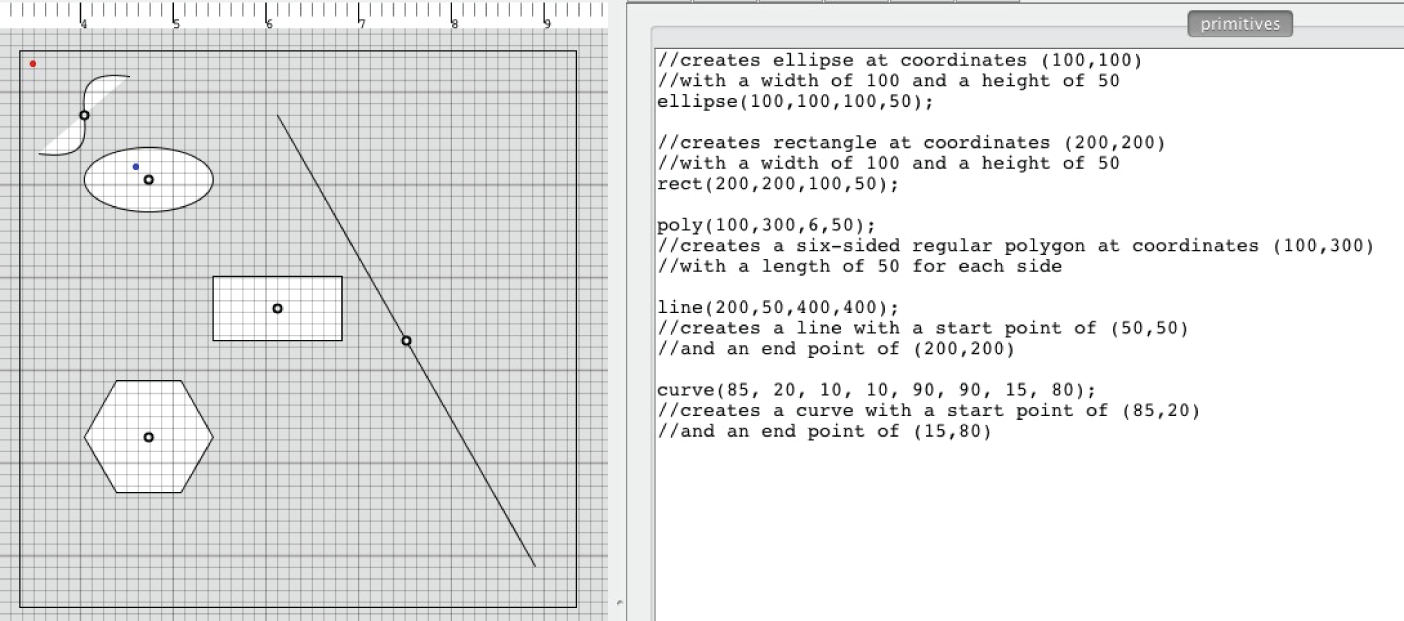
\includegraphics[width=6.5in]{images/primitives.png}
\caption{DressCode shape primitives with visible origins}
\label{fig:shape_primitives}
\end{figure}
\end{center} 

There is no required "draw" method for DressCode, as there are in many other graphics APIs, Instead all primitives are automatically drawn in the display panel in the order of their initialization, once the program has been run. In Soft Objects and Codeable Objects, when we required users to manually call draw method for any and all shapes in their program, they often forgot, and then had difficulty determining the reason why parts of their designs were not visible. 

Each shape primitive method returns an instance of the primitive it creates. A programmer can either create shapes with no reference as in figure \ref{fig:shape_primitives}, or they can assign them to an identifier at initialization, allowing them to reference and modify the shape later in the program. The shape transformation methods allow for a range of modifications to a shape, by passing a reference to the primitive the first argument, followed by different parameters for the modification, depending on the method (figure: \ref{fig:transformation}.) We began with a basic set of transformations, including move, rotate, methods that allowed for the modification of the stroke weight and color of the shape, and a hide method that prevented a primitive from being drawn. Based on our early user testing however, we gradually added in additional methods, based on what people wanted to do with their designs. This included a moveBy method, scale and mirroring functionality, a copy method, and an addition to the rotate method which allowed a shape to be rotated around a point other than its origin. 

 \begin{center}
\begin{figure}[h!]
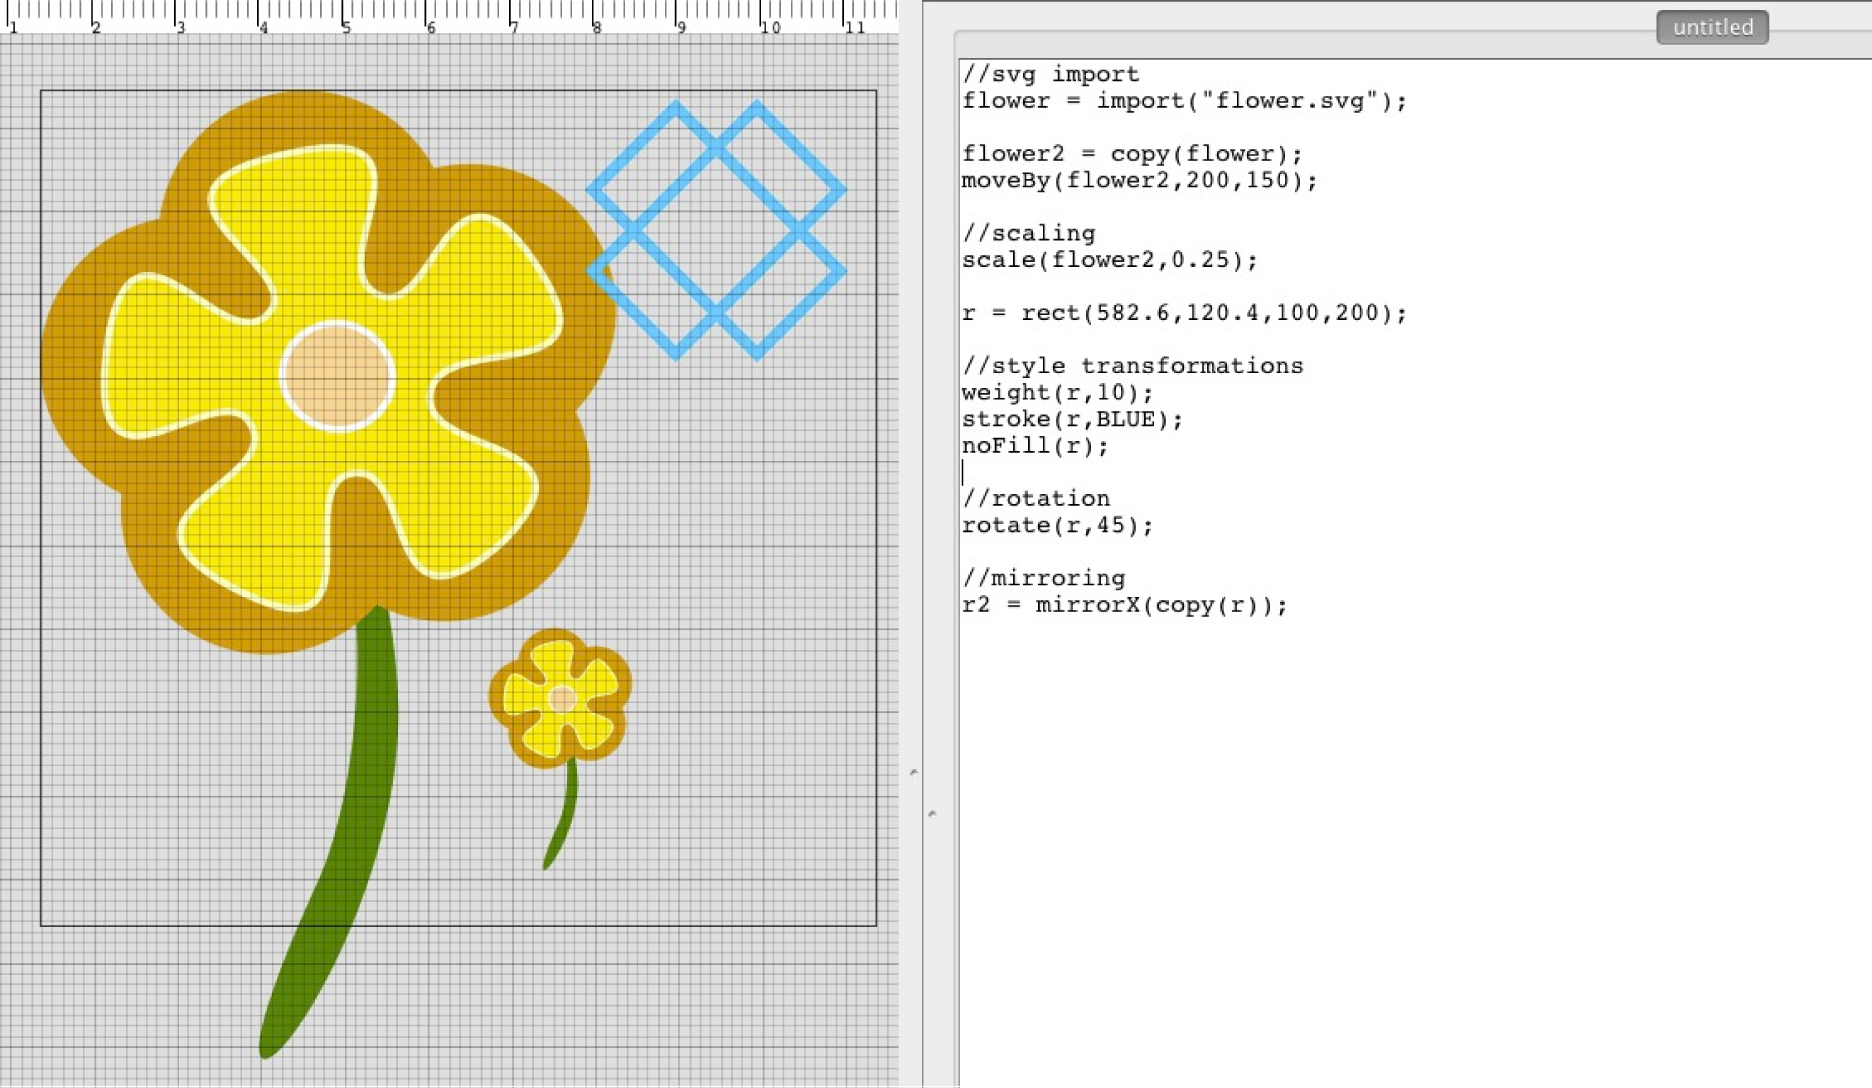
\includegraphics[width=6.5in]{images/transformation.png}
\caption{SVG import and sample of transformation methods}
\label{fig:transformation}
\end{figure}
\end{center} 

DressCode primitives can also be programmatically "grouped". Grouping provides an organizational structure for more complex configurations of primitives allows for the automatic transformations to multiple shapes. Groups have their own origin, which is used as the reference point for all move, rotation and scale methods applied to the group (figure: \ref{fig:grouping}.) For example, a collection of ellipses that is grouped and then moved to the center of the canvas would move the origin of the group to the center, and all the ellipses relative to the new origin. The origin of a group is automatically calculated as the centroid of all of the objects in the group and updated each time a primitive is added or removed. Groups are treated similarly to lists in that individual objects can be accessed and manipulated by via their index. Originally, primitives within a group were transformed relative to the origin of the group, however this caused confusion among many of our initial users. Each individual primitive is now translated according to the coordinate system of the canvas, regardless of whether it is in a group.

 \begin{center}
\begin{figure}[h!]
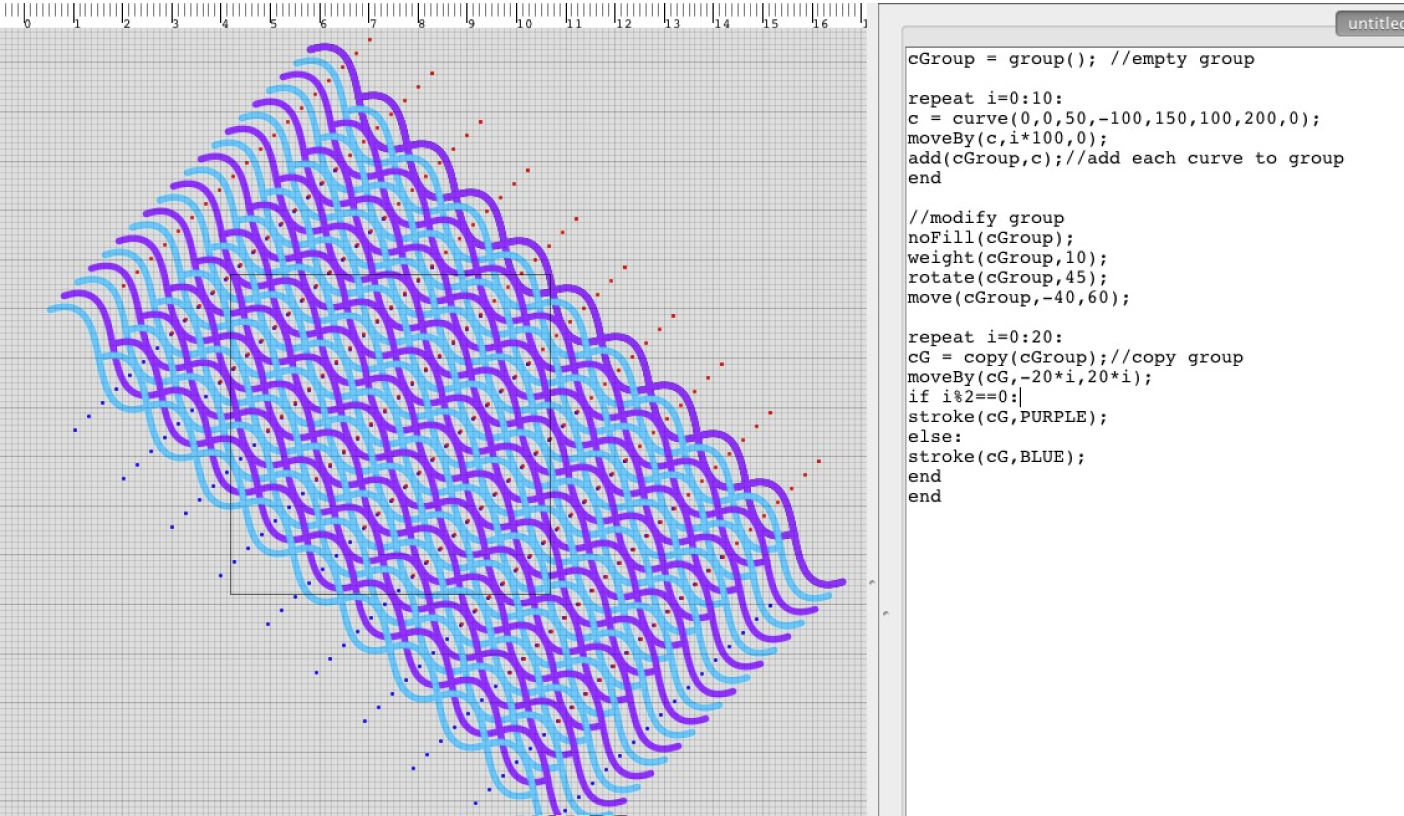
\includegraphics[width=6.5in]{images/grouping.png}
\caption{Grouping with transformation and repeat statements}
\label{fig:grouping}
\end{figure}
\end{center} 

\subsection{Interface Design}
The interface of DressCode has two primary sections, a design panel and a coding panel. The divider between the two panels can be resized, allowing the the 
\begin{center}
\begin{figure}[h!]
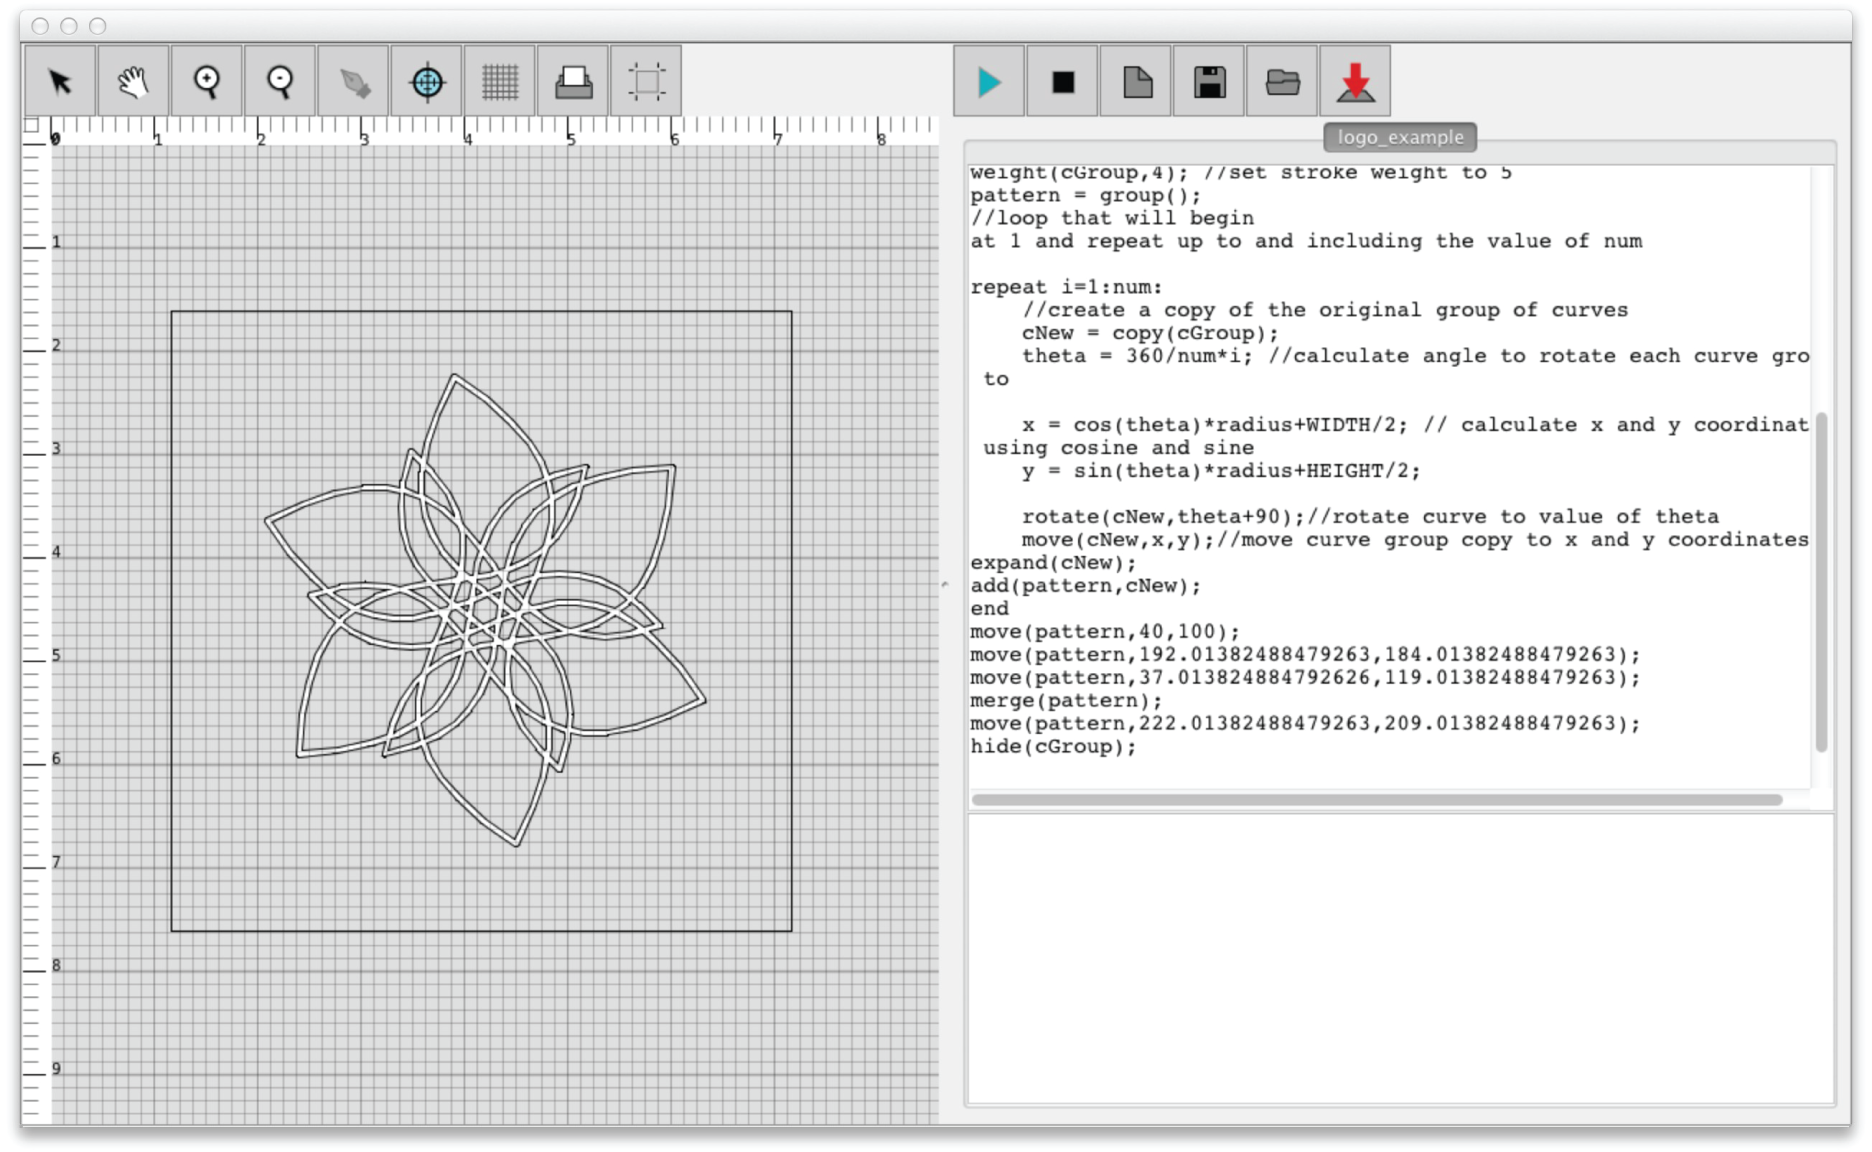
\includegraphics[width=6.5in]{images/dress_code_interface.png}
\caption{The DressCode interface}
\label{fig:dress_code_interface}
\end{figure}
\end{center}

  \begin{center}
\begin{figure}[h!]
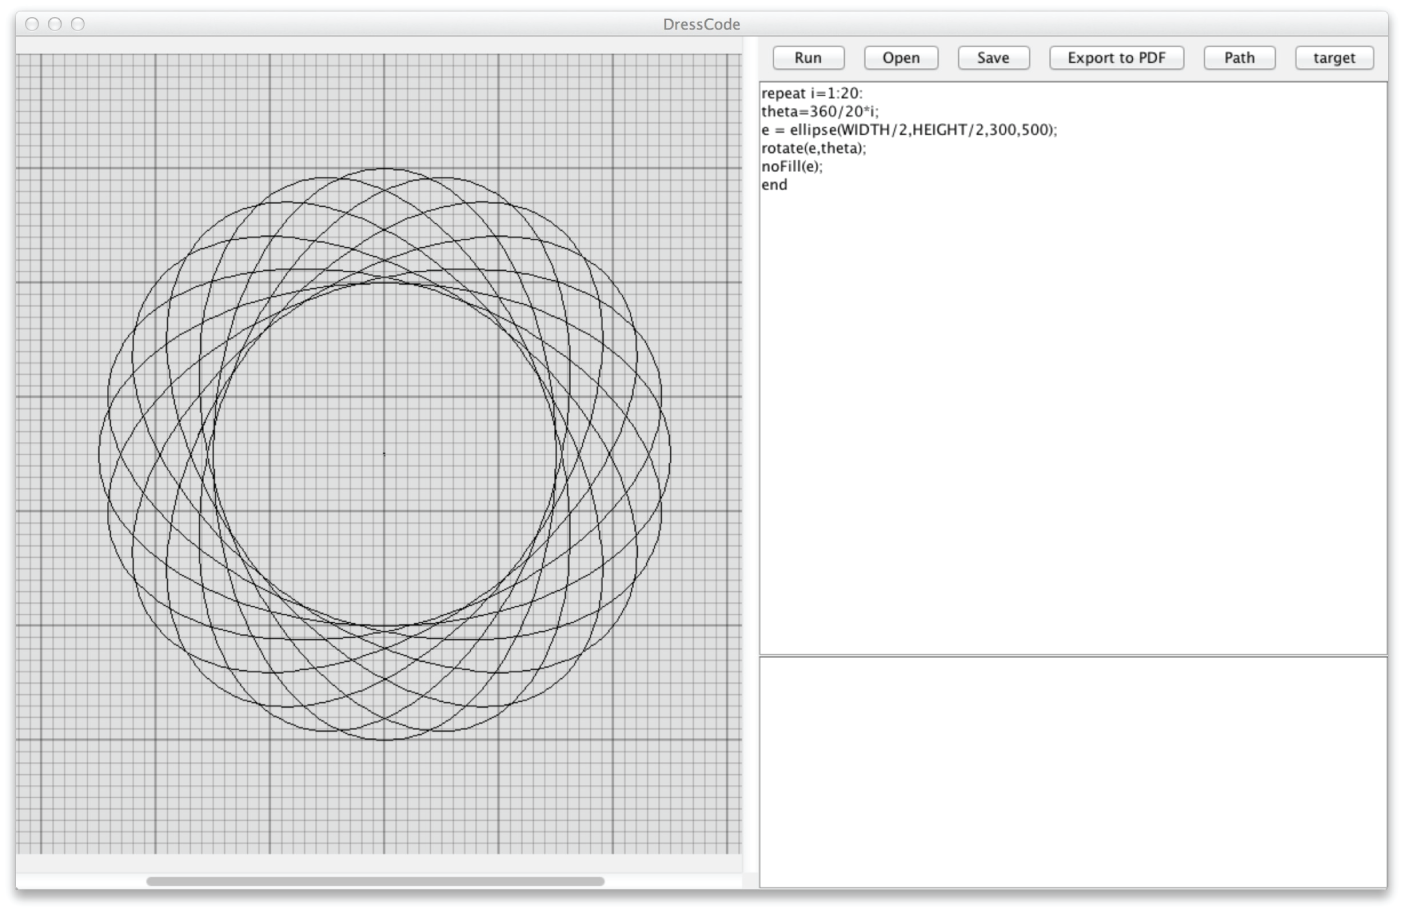
\includegraphics[width=6.5in]{images/early_dress_code.png}
\caption{The first bare-bones version of DressCode}
\label{fig:early_dress_code}
\end{figure}
\end{center}


\subsection{Fabrication process}

\section{Workshops}
\section{Results}
\section{Curriculum description}
\section{Preliminary curriculum results}
\section{Discussion}
\subsection{Starting notions of craft and computation}
\subsection{independent programming with a sense of ownership}
\subsection{Design Process and resultant aesthetics}
\subsection{Pride and Acomplishment in Algorithmic Craft}
\subsection{Design history and selection}
\subsection{Prototyping pt 2}
\subsection{Connection to other applications}

